\normaltrue \difficilefalse \tdifficilefalse
\correctiontrue

%\UPSTIidClasse{11} % 11 sup, 12 spé
%\newcommand{\UPSTIidClasse}{12}

\exer{Centrifugeuse des boues $\star$ \label{C2:06:33}}
\setcounter{question}{0}\UPSTIcompetence[2]{A3-05}
\UPSTIcompetence[2]{C2-06}
\index{Compétence C2-06}

\ifcorrection
\else
\marginnote{\textbf{Pas de corrigé pour cet exercice.}}
\fi

\ifprof
\else

La chaîne cinématique est représentée sur la figure
suivante.
\begin{center}
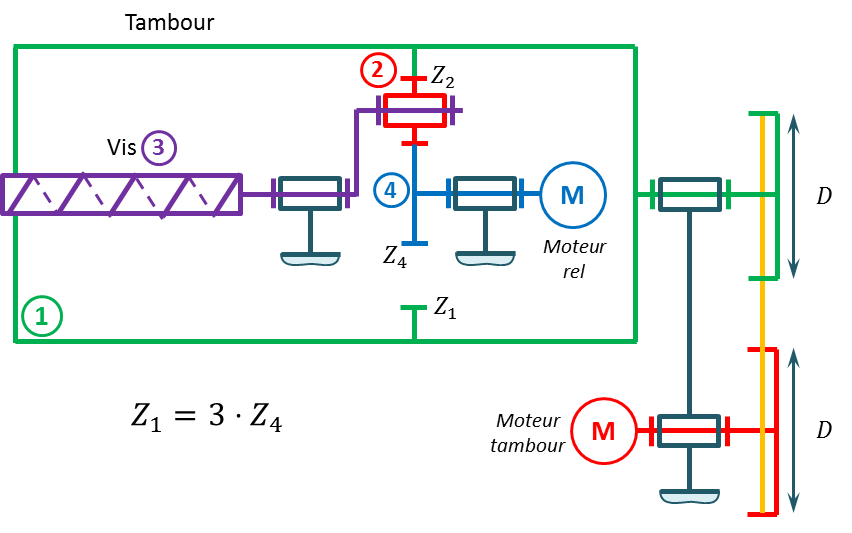
\includegraphics[width=\linewidth]{33_01}
\end{center}


La séquence de lancement de la centrifugeuse se déroule en trois phases :
\begin{itemize}
\item mise en marche du premier moteur $M_{\text{tambour}}$ jusqu’à ce que le tambour 1 atteigne sa vitesse
de consigne de 2 000 tours/min. Le moteur $M_{\text{rel}}$ est à l’arrêt;
\item mise en marche du deuxième moteur $M_{\text{rel}}$ jusqu’à ce que la vitesse différentielle de
2 tours/min soit atteinte entre le tambour 1 et la vis 3. La vis 3 tourne ainsi plus vite que le
tambour 1;
\item la boue liquide est ensuite introduite.
\end{itemize}
\fi


\question{Déterminer la fréquence de rotation de la vis (par rapport au bâti) lors de la phase de lancement.}
\ifprof
\else
\fi

\ifprof
\else
\begin{flushright}
\footnotesize{Corrigé  voir \ref{C2:06:33}.}
\end{flushright}%
\fi